% =====================================================================
% Guía del estudiante -- Álgebra 9° -- Trimestre I
% María Mercedes Cantillo · Colegio San Alberto Magno
% ---------------------------------------------------------------------
% Hilo conductor: Al-Juarismi y el nacimiento del álgebra
% Plan (etapas A y B): guia-periodo-I-reales-y-factorizacion.plan.md
% Temas (propuesta del trimestre I en curriculo/plan-anual.md, sesiones 005-022):
%   numerosreales, factorizacion, fraccionesecuaciones
% Cada \tema tiene \label{tema:...} para que las clases lo citen con
% \refguia{tema:...}. No borrar el .aux de esta guía.
% Ejercicios: SOLO reutilizados del banco (regla de la docente, 2026-09-15):
% radicacion-8, numeros-reales-8, irracionales-8, medidas-con-radicales-8,
% productos-notables-8, factorizacion-8, producto-polinomios-8, icfes.
% Única excepción: fracciones algebraicas, que no tenían NINGÚN ejercicio en el
% banco: 2 nuevos en fracciones-algebraicas-9.py (verificados con --sin-registro).
% Pendiente sin ejercicio: racionalización con denominador binomio (ver el plan).
%
% Compilar:  latexmk -pdf guia-periodo-I-reales-y-factorizacion.tex
% =====================================================================
\documentclass[11pt]{article}
\makeatletter\def\input@path{{../../../../plantillas/estilo/}}\makeatother
\usepackage{mmcantillo}

% ======================== DATOS DE LA GUÍA ============================
\tipodocumento{Guía del estudiante}
\asignatura{Álgebra}
\titulo{El libro que le dio nombre al álgebra}
\grado{9°}
\periodo{I}
\hiloconductor{Al-Juarismi y el nacimiento del álgebra}
% ======================================================================
% BORRADOR: el plan del trimestre está pendiente de aprobación de la docente (generación rápida 2026-09-14).
% DBA: matematicas grado 9 · DBA 1 — Utiliza los números reales (sus
%      operaciones, relaciones y propiedades) para resolver problemas con
%      expresiones polinómicas.
%      DBA 2 — Propone y desarrolla expresiones algebraicas en el conjunto de
%      los números reales y utiliza las propiedades de la igualdad y de orden
%      para determinar el conjunto solución de relaciones entre tales
%      expresiones.

\begin{document}

\encabezado

% ---------------------------------------------------------------------
% 1. Frase introductoria
% ---------------------------------------------------------------------
% verificado: https://archive.org/details/algebraofmohamme00khuwuoft — Rosen (1831), p. 3: «to compose a short work on Calculating by (the rules of) Completion and Reduction, confining it to what is easiest and most useful in arithmetic, such as men constantly require in cases of inheritance, legacies, partition, law-suits, and trade»
\frase{[Me animé] a componer un breve tratado sobre el cálculo por compleción
y reducción, limitándome a lo más fácil y más útil de la aritmética, lo que
los hombres necesitan constantemente en casos de herencias, legados,
particiones, pleitos y comercio.}
{Al-Juarismi, prólogo de su \emph{Álgebra} (trad. propia de la versión inglesa de F. Rosen, 1831)}

% ---------------------------------------------------------------------
% 2. Introducción
% ---------------------------------------------------------------------
\seccion{Introducción}

La palabra «álgebra» tiene más de mil años y viene del título de un libro
escrito en Bagdad por Muhammad ibn Musa al-Juarismi. Su autor quería enseñar
«lo más fácil y más útil» para repartir herencias, medir tierras y hacer
negocios, y lo hizo de una manera que hoy nos sorprende: sin letras ni
símbolos, solo con palabras y con dibujos de cuadrados y rectángulos.

Este trimestre seguiremos a Al-Juarismi. Empezaremos con una tablilla de
barro, mucho más antigua que su libro, donde un aprendiz de escriba escribió
una aproximación de $\sqrt{2}$: ¿qué tan buena es una aproximación?
Veremos cómo sus cuadrados y rectángulos explican los productos notables y la
factorización, y cómo su idea central —transformar una expresión sin cambiar
su valor— sirve para simplificar fracciones algebraicas y resolver ecuaciones.

\textbf{Al terminar este trimestre podrás:}
\begin{itemize}
  \item distinguir un valor exacto de una aproximación y calcular el error
        que se comete al aproximar;
  \item simplificar, operar y racionalizar expresiones con radicales;
  \item desarrollar productos notables y factorizar completamente un
        polinomio, apoyándote en modelos de área;
  \item simplificar y operar fracciones algebraicas, cuidando los valores
        para los que no están definidas;
  \item resolver ecuaciones factorizando y problemas que llevan a ellas.
\end{itemize}

Este trimestre trabaja dos Derechos Básicos de Aprendizaje del Ministerio de
Educación Nacional~\cite{mendba}:

\begin{dba}[Grado 9° · DBA 1]
Utiliza los números reales (sus operaciones, relaciones y propiedades) para
resolver problemas con expresiones polinómicas.
\end{dba}

\begin{dba}[Grado 9° · DBA 2]
Propone y desarrolla expresiones algebraicas en el conjunto de los números
reales y utiliza las propiedades de la igualdad y de orden para determinar
el conjunto solución de relaciones entre tales expresiones.
\end{dba}

% ---------------------------------------------------------------------
% 3. Marco teórico
% ---------------------------------------------------------------------
\seccion{Marco teórico}

\subsubsection*{Una tablilla de escuela}

En la Colección Babilónica de la Universidad de Yale hay una tablilla
redonda de barro, la \textbf{YBC 7289}, escrita en el sur de Mesopotamia (el
actual Irak) en el primer tercio del segundo milenio antes de Cristo. Tiene
dibujado un cuadrado con sus diagonales; en un lado está el número $30$ y
sobre la diagonal, en base $60$, los números $1;24,51,10$ y $42;25,35$. Por la
forma de la tablilla y la letra, los historiadores creen que es el ejercicio
de un aprendiz de escriba~\cite{fowler}.

\begin{center}
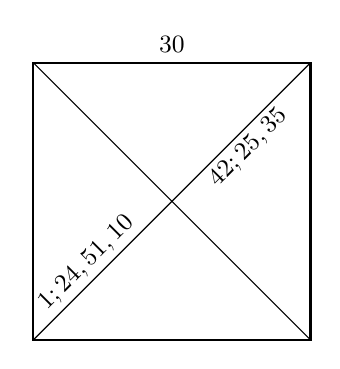
\begin{tikzpicture}[scale=1.1, every node/.style={font=\small}]
  \draw[thick] (0,0) rectangle (3.2,3.2);
  \draw (0,0) -- (3.2,3.2);
  \draw (0,3.2) -- (3.2,0);
  \node[above] at (1.6,3.2) {$30$};
  \node[rotate=45, above, inner sep=2pt] at (0.75,0.75) {$1;24,51,10$};
  \node[rotate=45, below, inner sep=2pt] at (2.35,2.35) {$42;25,35$};
\end{tikzpicture}

{\small Esquema de la tablilla YBC 7289 (los números están en base 60).}
\end{center}

El número $1;24,51,10$ significa
$1 + \frac{24}{60} + \frac{51}{60^2} + \frac{10}{60^3} = \num{1,41421296}\ldots$,
y $\sqrt{2} = \num{1,41421356}\ldots$: coinciden en sus primeras seis cifras.
Multiplicado por el lado, $30$, da la diagonal, $42;25,35$. Hace unos
3800 años ya se sabía que la diagonal de un cuadrado es su lado por un número
que \emph{no se puede escribir exactamente}, y se usaba una aproximación
excelente.

\subsubsection*{Bagdad y la Casa de la Sabiduría}

A comienzos del siglo IX, Bagdad era la capital del califato abasí. Allí, en
la Casa de la Sabiduría, un grupo de sabios traducía al árabe libros griegos e
indios de matemáticas y astronomía. Uno de ellos era \textbf{Muhammad ibn
Musa al-Juarismi} (hacia 780 – hacia 850). Bajo la protección del califa
al-Mamún, que gobernó desde el año 813, escribió un tratado que le dedicó:
\emph{Hisab al-jabr w'al-muqabala}, «cálculo por compleción y
equilibrio». De \emph{al-jabr} viene nuestra palabra \textbf{álgebra}, y de
su nombre, en la traducción latina de otro libro suyo (\emph{Algoritmi de
numero Indorum}), viene la palabra \textbf{algoritmo}~\cite{mactutorjuarismi}.

Su álgebra está escrita toda con palabras, sin un solo símbolo: la incógnita
se llama «la raíz» y su cuadrado, «el cuadrado». Aun así fue una revolución,
porque permitía tratar números racionales, irracionales y magnitudes
geométricas del mismo modo, como objetos que se suman, se multiplican y se
transforman~\cite{mactutorarabe}.

\subsubsection*{Resolver con figuras}

Al-Juarismi no solo daba la regla para resolver una ecuación: la demostraba
con un dibujo. Su ejemplo más famoso es «un cuadrado y diez raíces suyas
valen treinta y nueve», que hoy escribimos $x^2 + 10x = 39$. Pegaba al
cuadrado dos rectángulos, veía que al conjunto le faltaba una esquina
cuadrada y la completaba~\cite{rosen}. En el tema 2 haremos lo mismo.

\subsubsection*{Del álgebra de ecuaciones al álgebra moderna: Emmy Noether}

Mil años después, el álgebra ya no trataba solo de resolver ecuaciones, sino
de estudiar las estructuras donde se puede sumar y multiplicar. La gran
protagonista de ese cambio fue \textbf{Emmy Noether} (Erlangen, Alemania,
1882 – Bryn Mawr, Estados Unidos, 1935). En la Universidad de Gotinga, donde
llegó en 1915 invitada por Hilbert y Klein, escribió en 1921
\emph{Idealtheorie in Ringbereichen}, un artículo fundamental del álgebra
moderna; en 1918 ya había demostrado el teorema que relaciona las simetrías
de la física con las cantidades que se conservan. En 1933 los nazis la
expulsaron de la universidad y se fue a enseñar al Bryn Mawr College, en
Estados Unidos~\cite{mactutornoether}. Al morir ella, Albert Einstein
escribió:

% verificado: https://mathshistory.st-andrews.ac.uk/Obituaries/Noether_Emmy_Einstein/ — carta de Einstein al New York Times (4 may. 1935): «Pure mathematics is, in its way, the poetry of logical ideas»
\begin{cita}{Albert Einstein, carta a \emph{The New York Times} (1935), trad. propia~\cite{einstein}}
La matemática pura es, a su manera, la poesía de las ideas lógicas.
\end{cita}

% ---------------------------------------------------------------------
% 4. Temas
% ---------------------------------------------------------------------
\tema{Números reales: aproximación, error y radicales}\label{tema:numerosreales}

\begin{hilo}
El escriba de la tablilla YBC 7289 no podía escribir $\sqrt{2}$ exactamente,
y nosotros tampoco podemos escribir todas sus cifras. Siglos después,
Al-Juarismi operaba con raíces como con cualquier otro número. Aprendamos a
hacer las dos cosas: medir cuánto nos equivocamos al aproximar, y calcular
con las raíces exactas.
\end{hilo}

\begin{definicion}[Valor exacto, aproximación y error]
Un número real tiene un \textbf{valor exacto} ($\sqrt{2}$, $\pi$,
$\frac{1}{3}$) y muchas \textbf{aproximaciones} decimales ($\num{1,41}$,
$\num{3,14}$, $\num{0,333}$). Si $a$ aproxima a $x$:
\[
  \text{error absoluto} = |x - a|, \qquad
  \text{error relativo} = \frac{|x - a|}{|x|}\ \ (\text{suele darse en \%}).
\]
\end{definicion}

Con $\sqrt{2} \approx \num{1,41}$ el error absoluto es $\num{0,0042}$, y el
relativo, cerca del $\qty{0,3}{\percent}$. La tablilla babilónica se equivoca
en menos de una millonésima. Por eso escribir $\sqrt{5} = \num{2,23}$ es un
error: lo correcto es $\sqrt{5} \approx \num{2,24}$, con el signo $\approx$.

\subsubsection*{Construir raíces en la recta}

Con el teorema de Pitágoras (que estudias en Geometría) podemos construir
\emph{exactamente} la raíz de cualquier natural. La hipotenusa de un
triángulo rectángulo de catetos $3$ y $1$ mide $\sqrt{3^2 + 1^2} = \sqrt{10}$;
con el compás en $0$ la llevamos a la recta numérica. Con catetos $3$ y $2$
obtenemos $\sqrt{13}$. La construcción es exacta; la medida con la regla, no.

\subsubsection*{Radicales}

Para $a, b \ge 0$ se cumple $\sqrt{ab} = \sqrt{a}\,\sqrt{b}$ y, si $b > 0$,
$\sqrt{\frac{a}{b}} = \frac{\sqrt{a}}{\sqrt{b}}$. Con estas propiedades se
simplifican radicales sacando factores que son potencias exactas, y se suman
los radicales \textbf{semejantes} (con el mismo índice y el mismo radicando).

% Ejercicio: radicacion-8-035
\begin{ejemplo}[Radicales semejantes]
$5\sqrt{27} - \sqrt{147} + \sqrt{12} = 15\sqrt{3} - 7\sqrt{3} + 2\sqrt{3} =
10\sqrt{3}$, porque $27 = 9 \cdot 3$, $147 = 49 \cdot 3$ y $12 = 4 \cdot 3$.
\end{ejemplo}

\textbf{Racionalizar} es escribir una fracción equivalente sin raíces en el
denominador. Si el denominador es $\sqrt{b}$, se multiplica arriba y abajo
por $\sqrt{b}$; si es $\sqrt{a} - \sqrt{b}$, por su \textbf{conjugado}
$\sqrt{a} + \sqrt{b}$, porque
$(\sqrt{a} - \sqrt{b})(\sqrt{a} + \sqrt{b}) = a - b$.

% Ejercicio: radicacion-8-030
\begin{ejemplo}[Dividir radicales y racionalizar]
Con $a, b > 0$:
\[
  \sqrt{5a^3} \div \sqrt{24b^2} = \frac{a\sqrt{5a}}{2b\sqrt{6}}
  = \frac{a\sqrt{5a}\,\sqrt{6}}{2b\sqrt{6}\,\sqrt{6}} = \frac{a\sqrt{30a}}{12b}.
\]
\end{ejemplo}

\begin{aplicacion}[Planos exactos, obras aproximadas]
En un plano de arquitectura, la diagonal de una baldosa cuadrada de lado
$\qty{30}{cm}$ se escribe $30\sqrt{2}$~cm: es la medida exacta. En la obra,
el maestro corta con una cinta métrica que marca milímetros, así que usa una
aproximación. Decidir cuántas cifras de $\sqrt{2}$ hacen falta es decidir qué
error se puede tolerar: una baldosa admite un milímetro; la pieza de un motor,
mucho menos.
\end{aplicacion}

\begin{preguntas}
% Ejercicio: irracionales-8-013
\pregunta Las fracciones $\dfrac{7}{5}$, $\dfrac{17}{12}$ y $\dfrac{99}{70}$
se acercan cada vez más a $\sqrt{2}$. Eleva cada una al cuadrado y compara
con $2$; luego calcula, con la calculadora, cuánto se aleja cada una de
$\sqrt{2}$.
\espacio{3.5cm}
% Ejercicio: numeros-reales-8-013
\pregunta Representa en la recta real $\dfrac{1}{2} - (1 + \sqrt{2})$ y
constata que $\dfrac{1}{2} - (1 + \sqrt{2}) = \left(\dfrac{1}{2} - 1\right) - \sqrt{2}$.
Construye $\sqrt{2}$ con regla y compás.
\espacio{3cm}
% Ejercicio: radicacion-8-014, radicacion-8-036
\Needspace{6\baselineskip}
\pregunta Simplifica:
\begin{opciones*}(2)
  \item $\sqrt[3]{40}$
  \item $2\sqrt[3]{250} + \sqrt[3]{16} - 3\sqrt[3]{54}$
\end{opciones*}
\espacio{2.5cm}
% Ejercicio: numeros-reales-8-031, numeros-reales-8-033
\pregunta Efectúa en $\R$ y simplifica si es posible:
\begin{opciones*}(2)
  \item $\left(\sqrt{2} + \sqrt{5}\right)\left(\sqrt{3} + \sqrt{5}\right)$
  \item $\left(3 - \sqrt{2}\right)\left(1 - \sqrt{2}\right)$
\end{opciones*}
\espacio{2.5cm}
% Ejercicio: radicacion-8-031
\pregunta Escribe en la forma más simple, sin raíces en el denominador (las
letras representan números positivos): $2\sqrt[3]{27x^2} \div 3\sqrt[3]{16a^2b^4}$.
\espacio{3cm}
% Ejercicio: medidas-con-radicales-8-002
\pregunta En el triángulo isósceles $ABC$, la base $AB$ mide $10$~cm,
$BC = CA$ y la altura $CH$ mide $8$~cm ($CH$ es perpendicular a $AB$ y
$AH = HB$). Encuentra su perímetro exacto y una aproximación con dos cifras
decimales.
\espacio{3cm}
\end{preguntas}

\begin{resumen}
\begin{itemize}
  \item Una aproximación no es el número: se escribe con $\approx$, y su
        error absoluto es $|x - a|$; el relativo, $|x - a|/|x|$.
  \item $\sqrt{ab} = \sqrt{a}\,\sqrt{b}$ ($a, b \ge 0$): así se simplifican
        radicales; solo se suman los radicales semejantes.
  \item Para racionalizar se multiplica por $\sqrt{b}$ o por el conjugado,
        usando $(\sqrt{a} - \sqrt{b})(\sqrt{a} + \sqrt{b}) = a - b$.
\end{itemize}
\end{resumen}

% ---------------------------------------------------------------------
\tema{Productos notables y factorización}\label{tema:factorizacion}

\begin{hilo}
Al-Juarismi pensaba cada producto como un área: el cuadrado de «la raíz» es
un cuadrado de verdad, y «diez raíces» son rectángulos de ancho $10$ y largo
$x$. Con esos dibujos, los productos notables se ven y la factorización
consiste en armar un rectángulo con las piezas.
\end{hilo}

Un \textbf{producto notable} es un producto que se desarrolla con una regla
fija; \textbf{factorizar} es el camino inverso: escribir un polinomio como
producto. Los modelos de área muestran por qué funcionan las reglas.

% Ejercicio: factorizacion-8-264
\begin{ejemplo}[Un rectángulo hecho de cuatro piezas]
Un rectángulo de lados $x + 3$ y $x + 4$ se divide en cuatro rectángulos de
áreas $x^2$, $3x$, $4x$ y $12$. Sumando las piezas:
$(x + 3)(x + 4) = x^2 + 3x + 4x + 12 = x^2 + 7x + 12$. Leído al revés,
factorizar $x^2 + 7x + 12$ es encontrar los lados del rectángulo.

\begin{center}
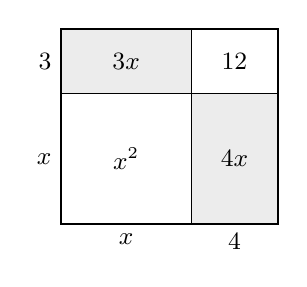
\begin{tikzpicture}[scale=0.55, every node/.style={font=\small}]
  \fill[gray!15] (3,0) rectangle (5,3);
  \fill[gray!15] (0,3) rectangle (3,4.5);
  \draw[thick] (0,0) rectangle (5,4.5);
  \draw (3,0) -- (3,4.5);
  \draw (0,3) -- (5,3);
  \node at (1.5,1.5) {$x^2$};
  \node at (4,1.5) {$4x$};
  \node at (1.5,3.75) {$3x$};
  \node at (4,3.75) {$12$};
  \node[below] at (1.5,0) {$x$};
  \node[below] at (4,0) {$4$};
  \node[left] at (0,1.5) {$x$};
  \node[left] at (0,3.75) {$3$};
\end{tikzpicture}
\end{center}
\end{ejemplo}

\begin{teorema}[Productos notables]
\[
  (a + b)^2 = a^2 + 2ab + b^2, \qquad
  (a + b)(a - b) = a^2 - b^2, \qquad
  (a + b)^3 = a^3 + 3a^2b + 3ab^2 + b^3.
\]
\end{teorema}

% Ejercicio: numeros-reales-8-036, productos-notables-8-043
\begin{ejemplo}[Dos productos notables]
$(a + b)(a - b) = a^2 - ab + ab - b^2 = a^2 - b^2$: los términos del medio se
cancelan. Y con el cubo de un binomio,
$(2a + 1)^3 = 8a^3 + 12a^2 + 6a + 1$.
\end{ejemplo}

\subsubsection*{Completar el cuadrado, como Al-Juarismi}

Para «un cuadrado y diez raíces suyas valen treinta y nueve»
($x^2 + 10x = 39$), Al-Juarismi da esta receta: toma la mitad de las raíces,
$5$; multiplícala por sí misma, $25$; súmale $39$, y da $64$; su raíz es $8$;
réstale la mitad de las raíces, $5$, y queda $3$: esa es la raíz, y el
cuadrado es $9$~\cite{rosen}. Y la demuestra con una figura: parte las diez
raíces en dos rectángulos de $5 \times x$ y los pega a dos lados del cuadrado
$x^2$. La figura casi es un cuadrado de lado $x + 5$; le falta una esquina de
$5 \times 5 = 25$. Si la agregamos a los dos lados de la igualdad, queda
$(x + 5)^2 = 39 + 25 = 64$: el lado grande mide $8$ y el pequeño,
$8 - 5 = 3$.

\begin{center}
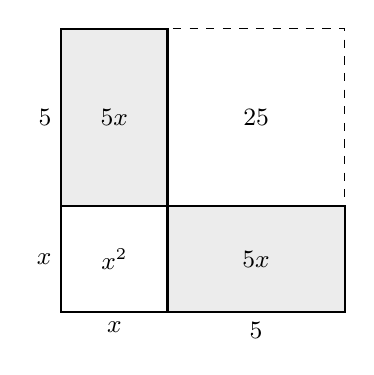
\begin{tikzpicture}[scale=0.45, every node/.style={font=\small}]
  \draw[thick] (0,0) rectangle (3,3);
  \fill[gray!15] (3,0) rectangle (8,3);
  \fill[gray!15] (0,3) rectangle (3,8);
  \draw[thick] (3,0) rectangle (8,3);
  \draw[thick] (0,3) rectangle (3,8);
  \draw[dashed] (3,3) rectangle (8,8);
  \node at (1.5,1.5) {$x^2$};
  \node at (5.5,1.5) {$5x$};
  \node at (1.5,5.5) {$5x$};
  \node at (5.5,5.5) {$25$};
  \node[below] at (1.5,0) {$x$};
  \node[below] at (5.5,0) {$5$};
  \node[left] at (0,1.5) {$x$};
  \node[left] at (0,5.5) {$5$};
\end{tikzpicture}

{\small La esquina punteada ($5 \times 5$) completa el cuadrado de lado $x + 5$.}
\end{center}

\subsubsection*{Los casos de factorización}

En la semana de refuerzo repasaste el factor común, la diferencia de
cuadrados, el trinomio cuadrado perfecto y el trinomio $x^2 + bx + c$. Ahora
completamos la lista:

\begin{itemize}
  \item \textbf{Trinomio $ax^2 + bx + c$:} se buscan dos números cuyo
        producto sea $a \cdot c$ y cuya suma sea $b$; con ellos se parte el
        término del medio y se agrupa.
  \item \textbf{Agrupación:} se forman grupos con un factor común, y el
        paréntesis que se repite se saca como factor.
  \item \textbf{Suma y diferencia de cubos:}
        $a^3 + b^3 = (a + b)(a^2 - ab + b^2)$ y
        $a^3 - b^3 = (a - b)(a^2 + ab + b^2)$.
  \item \textbf{Factorización completa:} se aplica primero el factor común y
        después los demás casos, hasta que ningún factor se pueda
        factorizar más.
\end{itemize}

% Ejercicio: factorizacion-8-226
\begin{ejemplo}[Trinomio $ax^2 + bx + c$]
En $4x^2 + 8x + 3$, $a \cdot c = 12$; dos números con producto $12$ y suma
$8$ son $6$ y $2$. Entonces
$4x^2 + 6x + 2x + 3 = 2x(2x + 3) + (2x + 3) = (2x + 1)(2x + 3)$.
\end{ejemplo}

% Ejercicio: factorizacion-8-109
\begin{ejemplo}[Agrupar y combinar casos]
$n^3 + 2n^2 - 4n - 8 = n^2(n + 2) - 4(n + 2) = (n + 2)(n^2 - 4)
= (n + 2)(n + 2)(n - 2) = (n + 2)^2(n - 2)$. Después de agrupar apareció una
diferencia de cuadrados: la factorización no termina hasta que no queda nada
por factorizar.
\end{ejemplo}

\begin{aplicacion}[Cajas de cartón]
Para hacer una caja sin tapa se corta un cuadrado de lado $x$ en cada esquina
de una lámina y se doblan los bordes. Su volumen es un producto de tres
factores —largo, ancho y alto—, es decir, un polinomio de grado $3$ ya
factorizado. Las fábricas de empaques comparan así distintos cortes: cada
factor dice qué pasa con una medida, y el volumen es cero exactamente cuando
algún factor vale cero.
\end{aplicacion}

\begin{preguntas}
% Ejercicio: productos-notables-8-018, productos-notables-8-021, productos-notables-8-044
\pregunta Desarrolla aplicando los productos notables:
\begin{opciones*}(3)
  \item $(2a + 5)^2$
  \item $(8a - 3)^2$
  \item $(3a - 2)^3$
\end{opciones*}
\espacio{3cm}
% Ejercicio: factorizacion-8-222, factorizacion-8-223, factorizacion-8-230
\pregunta Factoriza:
\begin{opciones*}(3)
  \item $5x^2 - 13x + 6$
  \item $2x^2 - x - 10$
  \item $2x^2 + x - 6$
\end{opciones*}
\espacio{3cm}
% Ejercicio: factorizacion-8-305, factorizacion-8-306, factorizacion-8-312
\pregunta Factoriza:
\begin{opciones*}(3)
  \item $a^3 + 1$
  \item $a^3 - 1$
  \item $1000h^3 + 27k^3$
\end{opciones*}
\espacio{3cm}
% Ejercicio: factorizacion-8-101, factorizacion-8-375, factorizacion-8-377, factorizacion-8-400
\pregunta Factoriza completamente:
\begin{opciones*}(2)
  \item $x^3 - 3x^2 - x + 3$
  \item $x^4 - 1$
  \item $18x - 8x^3$
  \item $12x^2y - 36xy^2 + 27y^3$
\end{opciones*}
\espacio{3cm}
% Ejercicio: factorizacion-8-158
\Needspace*{9\baselineskip}
\pregunta Explica si $(a + b)^2 = a^2 + b^2$. ¿Qué condiciones deben cumplir
$a$ y $b$ para que se cumpla esa igualdad? Dibuja el modelo de área para
justificar tu respuesta.
\espacio{3cm}
% Ejercicio: productos-notables-8-099
\pregunta Determina el volumen de un cubo cuya arista mide $3a - 2$
centímetros, con $a > \frac{2}{3}$.
\espacio{2cm}
% Ejercicio: factorizacion-8-262
\Needspace{6\baselineskip}
\pregunta Un rectángulo tiene área $x^2 + 5x + 4$ y lados $x + \ ?$ y
$x + \ ?$. Los valores correctos de los signos de interrogación son:
\begin{opciones*}(4)
  \item $-4$ y $-1$
  \item $4$ y $-1$
  \item $-4$ y $1$
  \item $4$ y $1$
\end{opciones*}
\end{preguntas}

\begin{resumen}
\begin{itemize}
  \item $(a + b)^2 = a^2 + 2ab + b^2$, $(a + b)(a - b) = a^2 - b^2$,
        $(a + b)^3 = a^3 + 3a^2b + 3ab^2 + b^3$; los modelos de área
        muestran por qué.
  \item Completar el cuadrado, como Al-Juarismi: $x^2 + 10x$ más la esquina
        $25$ es $(x + 5)^2$.
  \item Para factorizar completamente: primero el factor común, después los
        casos (trinomios, agrupación, cubos), hasta que nada se pueda
        factorizar más.
\end{itemize}
\end{resumen}

% ---------------------------------------------------------------------
\tema{Fracciones algebraicas y ecuaciones}\label{tema:fraccionesecuaciones}

\begin{hilo}
El título del libro de Al-Juarismi habla de \emph{compleción} y
\emph{equilibrio}: transformar una igualdad sin romperla, haciendo lo mismo
en los dos lados. Esa es la idea de este tema: transformar fracciones y
ecuaciones sin cambiar su valor, y cuidar lo que se pierde en el camino,
como las soluciones negativas que él nunca aceptó.
\end{hilo}

\begin{definicion}[Fracción algebraica]
Una \textbf{fracción algebraica} es un cociente $\dfrac{P(x)}{Q(x)}$ de dos
polinomios. No está definida en los valores de $x$ que anulan el
denominador: esos son los \textbf{valores excluidos}.
\end{definicion}

Para \textbf{simplificar}, se factorizan el numerador y el denominador y se
cancelan los \emph{factores} comunes (nunca los sumandos). Los valores
excluidos se buscan en la fracción \emph{original}, antes de cancelar.

% Ejercicio: fracciones-algebraicas-9-001 (literal a)
\begin{ejemplo}[Simplificar]
\[
  \frac{x^2 - 9}{x^2 + 3x} = \frac{(x - 3)(x + 3)}{x(x + 3)} = \frac{x - 3}{x},
  \qquad x \ne 0,\ x \ne -3.
\]
\end{ejemplo}

Las fracciones algebraicas se operan como las numéricas: para multiplicar,
se factoriza todo y se cancela; para dividir, se multiplica por la fracción
invertida; para sumar o restar, se busca un denominador común, que se arma
con los factores de los denominadores.

% Ejercicio: fracciones-algebraicas-9-002 (literales a y c)
\begin{ejemplo}[Multiplicar y sumar]
\[
  \frac{x^2 - 1}{x + 2} \cdot \frac{x^2 + 4x + 4}{x - 1}
  = \frac{(x - 1)(x + 1)}{x + 2} \cdot \frac{(x + 2)^2}{x - 1} = (x + 1)(x + 2),
\]
\[
  \frac{1}{x - 1} + \frac{2}{x + 1}
  = \frac{(x + 1) + 2(x - 1)}{(x - 1)(x + 1)} = \frac{3x - 1}{x^2 - 1}.
\]
\end{ejemplo}

\subsubsection*{Ecuaciones que se resuelven factorizando}

\begin{teorema}[Producto cero]
Si $A \cdot B = 0$, entonces $A = 0$ o $B = 0$.
\end{teorema}

Por eso, para resolver una ecuación se pasan todos los términos a un lado,
se factoriza y se iguala cada factor a cero. \textbf{Cuidado:} no se debe
dividir entre una expresión que contenga la incógnita, porque se pueden
perder soluciones.

% Ejercicio: factorizacion-8-376
\begin{ejemplo}[Una ecuación por factorización]
Como $m^2 - 5m + 6 = (m - 2)(m - 3)$, la ecuación $m^2 - 5m + 6 = 0$ equivale
a $(m - 2)(m - 3) = 0$: $m = 2$ o $m = 3$.
\end{ejemplo}

\begin{aplicacion}[Cuando la respuesta tiene que tener sentido]
En los problemas de medidas, la ecuación puede tener soluciones que el
problema no admite: una longitud negativa, un radio igual a cero o un valor
que anula un denominador. Como Al-Juarismi, que buscaba el lado de un
cuadrado, hay que volver al enunciado y decidir cuáles soluciones responden
la pregunta.
\end{aplicacion}

\begin{preguntas}
% Ejercicio: fracciones-algebraicas-9-001 (literales b, c y d)
\pregunta Simplifica e indica los valores de $x$ para los que la expresión
no está definida:
\begin{opciones*}(3)
  \item $\dfrac{x^2 - 4}{x^2 - 4x + 4}$
  \item $\dfrac{2x^2 + 6x}{x^2 - 9}$
  \item $\dfrac{x^3 - 1}{x^2 - 1}$
\end{opciones*}
\espacio{3.5cm}
% Ejercicio: fracciones-algebraicas-9-002 (literales b y d)
\pregunta Efectúa y simplifica:
\begin{opciones*}(2)
  \item $\dfrac{x^2 - x - 6}{x^2 - 4} \div \dfrac{x - 3}{x + 2}$
  \item $\dfrac{x}{x^2 - 9} - \dfrac{1}{x - 3}$
\end{opciones*}
\espacio{3.5cm}
% Ejercicio: factorizacion-8-155
\pregunta El perímetro de un círculo, medido en centímetros, y su área,
medida en centímetros cuadrados, tienen el mismo valor numérico. Plantea una
ecuación y resuélvela factorizando: ¿cuánto mide el radio?
\espacio{3cm}
% Ejercicio: factorizacion-8-156
\pregunta El volumen de un cubo de arista $a$, medido en centímetros cúbicos,
y el área total de sus seis caras, medida en centímetros cuadrados, tienen el
mismo valor numérico. Plantea una ecuación y resuélvela factorizando:
¿cuánto mide la arista?
\espacio{3cm}
% Ejercicio: icfes-cuadernillo-2026-031 (textual, © Icfes 2026)
\Needspace{14\baselineskip}
\pregunta Un profesor de Matemáticas les pide a sus estudiantes solucionar la
siguiente ecuación: $(x + 2)(x + 3) = 5(x + 3)$. María, Nelson y Óscar
realizan, cada uno, los siguientes procedimientos:
\begin{center}
\small
\begin{tabular}{lll}
\textbf{María} & \textbf{Nelson} & \textbf{Óscar} \\
$x^2 + 5x + 6 = 5x + 15$ & $(x + 2)(x + 3) - 5(x + 3) = 0$ & $x + 2 + x + 3 = 5 + x + 3$ \\
$x^2 + 6 = 15$ & $(x + 3)[(x + 2) - 5] = 0$ & $2x + 5 = x + 8$ \\
$x^2 = 15 - 6$ & $(x + 3)(x - 3) = 0$ & $2x - x = 8 - 5$ \\
$x^2 = 9$ & $x^2 - 9 = 0$ & $x = 3$ \\
$x = \pm 3$ & $x^2 = 9$ & \\
 & $x = \pm 3$ & \\
\end{tabular}
\end{center}
¿Cuál(es) estudiante(s) desarrolló(aron) un procedimiento correcto para
solucionar la ecuación? {\small (Icfes, 2026~\cite{icfes})}
\begin{opciones*}(2)
  \item Solo Nelson y Óscar.
  \item Solo María y Nelson.
  \item Solamente Óscar.
  \item Solamente María.
\end{opciones*}
\end{preguntas}

\begin{resumen}
\begin{itemize}
  \item Una fracción algebraica no está definida donde se anula su
        denominador; se simplifica cancelando factores, no sumandos.
  \item Se multiplican, dividen, suman y restan como las fracciones
        numéricas, factorizando primero.
  \item Si $A \cdot B = 0$, entonces $A = 0$ o $B = 0$. No se divide entre
        la incógnita, y al final se revisa qué soluciones tienen sentido.
\end{itemize}
\end{resumen}

% ---------------------------------------------------------------------
% 5. Prepárate para Saber 11
% ---------------------------------------------------------------------
\seccion{Prepárate para Saber 11}

Marca la respuesta correcta. Cada pregunta tiene una sola opción válida.

\begin{preguntas}
% Ejercicio: icfes-cuadernillo-2026-027 (textual, © Icfes 2026)
\pregunta Una prueba atlética tiene un récord mundial de 10,49 segundos y un
récord olímpico de 10,50 segundos. ¿Es posible que un atleta registre un
tiempo, en el mismo tipo de prueba, que rompa el récord olímpico pero no el
mundial? {\small (Icfes, 2026~\cite{icfes})}
\begin{opciones}
  \item Sí, porque puede registrar, por ejemplo, un tiempo de 10,497
        segundos, que está entre los dos tiempos récord.
  \item Sí, porque puede registrar un tiempo menor que 10,4 y marcaría un
        nuevo récord.
  \item No, porque no existe un registro posible entre los dos tiempos
        récord.
  \item No, porque cualquier registro menor que el récord olímpico va a ser
        menor que el récord mundial.
\end{opciones}
% Ejercicio: producto-polinomios-8-124
\pregunta Al-Juarismi escribía: «He partido diez en dos porciones. He
multiplicado una de las dos porciones por la otra. Después he multiplicado
una de las dos por sí misma, y el producto de la multiplicación por sí misma
es cuatro veces el producto de una por la otra». En notación moderna: si las
porciones son $x$ y $10 - x$, su producto es $x(10 - x) = 10x - x^2$ y el
producto de $x$ por sí misma es $x^2$, así que $x^2 = 4(10x - x^2)$. Sumando
$4x^2$ en ambos lados queda $5x^2 = 40x$, y dividiendo por $5x$ se obtiene
$x = 8$. Las porciones en las que se divide $10$ de acuerdo con el método de
Al-Juarismi son:
\begin{opciones*}(4)
  \item $9$ y $1$
  \item $8$ y $2$
  \item $6$ y $4$
  \item $10$ y $0$
\end{opciones*}
% Ejercicio: factorizacion-8-373
\pregunta Una diferencia de cubos se puede ver con volúmenes: a un cubo de
arista $x$ se le quita un cubo de arista $y$ y lo que queda se parte en tres
cajas, lo que da
$x^3 - y^3 = (x - y)x^2 + (x - y)xy + (x - y)y^2 = (x - y)\left(x^2 + xy + y^2\right)$.
En esa igualdad, cada uno de los sumandos representa:
\begin{opciones}
  \item El área de las caras laterales de las cajas.
  \item La longitud de los lados de las cajas.
  \item El volumen de las cajas.
  \item El volumen de dos de las cajas y el área de la más pequeña.
\end{opciones}
% Ejercicio: productos-notables-8-122
\pregunta Considera un cubo de arista $a$. Si se duplica su arista, el
volumen del cubo obtenido es:
\begin{opciones*}(4)
  \item $2a^3$
  \item $4a^3$
  \item $6a^3$
  \item $8a^3$
\end{opciones*}
\end{preguntas}

% ---------------------------------------------------------------------
% 6. Cierre del hilo conductor
% ---------------------------------------------------------------------
\seccion{Cierre: de la tablilla al álgebra moderna}

Un aprendiz de escriba en Mesopotamia aproximó $\sqrt{2}$ con seis cifras
correctas. Dos mil quinientos años después, en Bagdad, Al-Juarismi resolvió
ecuaciones con cuadrados y rectángulos y le dio nombre al álgebra. Mil años
más tarde, Emmy Noether convirtió el álgebra en el estudio de estructuras.
En este trimestre recorriste ese camino en pequeño: aproximaste y mediste
errores, operaste con radicales, factorizaste con modelos de área y
resolviste ecuaciones transformándolas sin cambiar su valor. En el siguiente
trimestre usaremos esas herramientas para estudiar la primera función, la
lineal, y los sistemas de ecuaciones; y en el tercero volveremos a completar
el cuadrado de Al-Juarismi para llegar a la fórmula de la ecuación
cuadrática.

% ---------------------------------------------------------------------
% 7. Evaluación (secciones institucionales)
% ---------------------------------------------------------------------
\clearpage
\matrizevaluacion
  {Distingue entre valor exacto y aproximación; reconoce los productos
   notables, los casos de factorización y los valores excluidos de una
   fracción algebraica.}
  {Calcula errores de aproximación; simplifica, opera y racionaliza
   radicales; factoriza completamente; opera fracciones algebraicas y
   resuelve ecuaciones por factorización.}
  {Comprueba sus resultados sustituyendo valores o midiendo el error, y
   corrige sus procedimientos cuando encuentra una contradicción.}
  {Reconoce que el álgebra es obra de culturas y personas muy distintas
   —escribas babilonios, sabios de Bagdad, mujeres como Emmy Noether— y
   valora el aporte de sus compañeros al discutir un procedimiento.}

\autoevaluacion

\seguimientodocente

% ---------------------------------------------------------------------
% 8. Referencias
% ---------------------------------------------------------------------
\begin{referencias}
% verificado: https://mathshistory.st-andrews.ac.uk/Obituaries/Noether_Emmy_Einstein/ — carta de Einstein al New York Times, publicada el 4 de mayo de 1935
\bibitem{einstein} Einstein, A. (1935, 4 de mayo). The late Emmy Noether
  [Carta al editor]. \emph{The New York Times}.
% verificado: https://www.sciencedirect.com/science/article/pii/S0315086098922091 — Historia Mathematica 25 (1998), 366–378 (PDF: https://www.ux1.eiu.edu/~cidelman/Classes/4900/Class%20Notes/Babylonian%20Approximations.pdf): YBC 7289, lado 30, 1;24,51,10 y 42;25,35, ejercicio escolar, primer tercio del II milenio a. C.
\bibitem{fowler} Fowler, D. y Robson, E. (1998). Square root approximations
  in Old Babylonian mathematics: YBC 7289 in context. \emph{Historia
  Mathematica}, 25(4), 366--378.
% verificado: recursos/matematicas/icfes/09-Marzo_Cuadernillo-de-Preguntas-Matematicas-Saber-11-2026.pdf (archivo local) — preguntas 27 y 31, transcritas textualmente en recursos/banco/matematicas/icfes-cuadernillo-2026.py
\bibitem{icfes} Icfes (2026). \emph{Cuadernillo de preguntas, Prueba de
  Matemáticas, Saber 11.\textsuperscript{o}}. Bogotá: Icfes. Preguntas 27 y 31
  (uso académico con crédito).
% verificado: https://gblumen.mineducacion.gov.co/cgi-bin/koha/opac-detail.pl?biblionumber=4785 — MEN 2016, ISBN 978-958-691-913-5
\bibitem{mendba} Ministerio de Educación Nacional (2016). \emph{Derechos
  Básicos de Aprendizaje V.2: Matemáticas}. Bogotá: MEN.
% verificado: https://mathshistory.st-andrews.ac.uk/HistTopics/Arabic_mathematics/ — el álgebra de al-Juarismi permitía tratar racionales, irracionales y magnitudes geométricas como «objetos algebraicos»
\bibitem{mactutorarabe} O'Connor, J. J. y Robertson, E. F. \emph{Arabic
  mathematics: forgotten brilliance?} MacTutor History of Mathematics,
  Universidad de St Andrews.
% verificado: https://mathshistory.st-andrews.ac.uk/Biographies/Al-Khwarizmi/ — Casa de la Sabiduría; al-Mamún califa desde 813; le dedicó el tratado de álgebra; Hisab al-jabr w'al-muqabala; «algebra» y «algorithm» (Algoritmi de numero Indorum); todo en palabras; c. 780 – c. 850
\bibitem{mactutorjuarismi} O'Connor, J. J. y Robertson, E. F.
  \emph{Abu Ja'far Muhammad ibn Musa Al-Khwarizmi}. MacTutor History of
  Mathematics, Universidad de St Andrews.
% verificado: https://mathshistory.st-andrews.ac.uk/Biographies/Noether_Emmy/ — Erlangen 1882 – Bryn Mawr 1935; Gotinga desde 1915 (Hilbert y Klein); teorema de 1918; Idealtheorie in Ringbereichen (1921); expulsada en 1933, Bryn Mawr College
\bibitem{mactutornoether} O'Connor, J. J. y Robertson, E. F. \emph{Emmy
  Amalie Noether}. MacTutor History of Mathematics, Universidad de St
  Andrews.
% verificado: https://archive.org/details/algebraofmohamme00khuwuoft — Londres, Oriental Translation Fund, 1831; dedicatoria a al-Mamún y propósito del libro (p. 3); x² + 10x = 39 (p. 8) y su demostración con figuras (pp. 13–15)
\bibitem{rosen} Rosen, F. (ed. y trad.) (1831). \emph{The Algebra of
  Mohammed ben Musa}. Londres: Oriental Translation Fund.
\end{referencias}

\end{document}
